\makeatletter
\let\pd@OrigRequirePackage\RequirePackage
\def\pd@dvipsname{dvips}
\def\RequirePackage{\@ifnextchar[\pd@RP@i{\pd@RP@i[\@empty]}}
\def\pd@RP@i[#1]#2{\@ifnextchar[{\pd@RP@ii{#1}{#2}}{\pd@RP@ii{#1}{#2}[\@empty]}}
\def\pd@RP@ii#1#2[#3]{%
  \def\pd@rpname{#2}%
  \ifx\pd@rpname\pd@hyperrefname
    \def\pd@newopts{}%
    \def\pd@first{1}%
    \ifx#1\@empty\else
      \@for\pd@tempopt:=#1\do{%
        \ifx\pd@tempopt\pd@dvipsname\else
          \ifx\pd@first\@empty
            \edef\pd@newopts{\pd@newopts,\pd@tempopt}%
          \else
            \edef\pd@newopts{\pd@tempopt}%
            \def\pd@first{}%
          \fi
        \fi
      }%
    \fi
    \ifx#3\@empty
      \pd@OrigRequirePackage[\pd@newopts]{#2}%
    \else
      \pd@OrigRequirePackage[\pd@newopts]{#2}[#3]%
    \fi
  \else
    \ifx#3\@empty
      \pd@OrigRequirePackage[#1]{#2}%
    \else
      \pd@OrigRequirePackage[#1]{#2}[#3]%
    \fi
  \fi
}
\def\pd@hyperrefname{hyperref}
\def\c@lor@to@ps#1 #2\@@{}%
\def\pdfmark#1{}%
\makeatother
\documentclass[style=fyma,palette=blue]{powerdot}
\usepackage{amsmath,amssymb}
\usepackage{booktabs}
\usepackage{colortbl}
\usepackage[most]{tcolorbox}
\usepackage{tikz}
\usetikzlibrary{calc,positioning,shapes.geometric,backgrounds}
\usepackage{fontawesome5}

\definecolor{brandNavy}{RGB}{15,32,67}
\definecolor{brandTeal}{RGB}{0,168,150}
\definecolor{brandBlue}{RGB}{24,119,242}
\definecolor{brandGray}{RGB}{245,247,250}
\definecolor{brandAccent}{RGB}{230,81,0}

\tcbset{
  colback=brandGray,
  colframe=brandNavy,
  fonttitle=\bfseries,
  arc=3pt,
  boxrule=0.8pt,
  left=4pt,
  right=4pt,
  top=4pt,
  bottom=4pt
}

\title{\Huge Nexa Platform Architecture\\ \Large Next-Gen Enterprise AI \& Distributed Cloud Systems}
\author{Dr. Elena Vance \and Marcus Chen}
\date{\today}

\begin{document}

\maketitle

\begin{slide}{Executive Agenda}
\begin{itemize}
  \item \textbf{Strategic Overview}: Enterprise AI Requirements \& Market Vision
  \item \textbf{Platform Architecture}: Multi-Tier Microservice Mesh \& Neural Core
  \item \textbf{Security \& Governance}: Zero-Trust Encryption \& Compliance Framework
  \item \textbf{Performance Benchmarks}: Latency, Throughput \& SLA Targets
  \item \textbf{Deployment Models}: Multi-Region Cloud \& Edge Integration
  \item \textbf{Strategic Roadmap}: 2026--2027 Development \& Delivery Milestones
\end{itemize}
\end{slide}

\section{Strategic Overview}

\begin{slide}{Market Drivers \& Enterprise Challenges}
\begin{itemize}
  \item \textbf{Exponential Data Growth}: Enterprise telemetry data expanding at 45\% CAGR.
  \item \textbf{Legacy Bottlenecks}: Monolithic backends struggle with sub-50ms latency SLAs.
  \item \textbf{Regulatory Fragmentation}: Strict data sovereignty requirements across EU and APAC regions.
  \item \textbf{MLOps Complexity}: Inefficient model deployment pipelines increasing cloud compute costs.
\end{itemize}
\end{slide}

\begin{slide}{Nexa Core Value Proposition}
\begin{minipage}[t]{0.48\textwidth}
\begin{tcolorbox}[title=Legacy Architecture,colframe=red!70!black,colback=red!5]
\small
\begin{itemize}
  \item Monolithic limits
  \item P99 latency $>$ 250ms
  \item Manual failover
  \item Fragmented security
\end{itemize}
\end{tcolorbox}
\end{minipage}%
\hfill
\begin{minipage}[t]{0.48\textwidth}
\begin{tcolorbox}[title=Nexa Next-Gen Engine,colframe=brandTeal,colback=brandTeal!5]
\small
\begin{itemize}
  \item Autonomous scaling
  \item P99 latency $<$ 20ms
  \item Self-healing mesh
  \item Unified zero-trust
\end{itemize}
\end{tcolorbox}
\end{minipage}
\end{slide}

\section{Enterprise Architecture}

\begin{slide}{Multi-Tier Microservice Mesh}
\begin{center}
\small
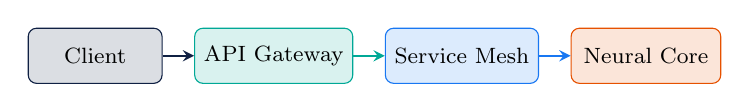
\begin{tikzpicture}[node distance=0.4cm, auto, >=stealth]
  \node[draw=brandNavy, fill=brandNavy!15, rectangle, rounded corners=3pt, minimum width=1.7cm, minimum height=0.7cm] (client) {\footnotesize Client};
  \node[draw=brandTeal, fill=brandTeal!15, rectangle, rounded corners=3pt, minimum width=1.9cm, minimum height=0.7cm, right=of client] (gw) {\footnotesize API Gateway};
  \node[draw=brandBlue, fill=brandBlue!15, rectangle, rounded corners=3pt, minimum width=1.9cm, minimum height=0.7cm, right=of gw] (mesh) {\footnotesize Service Mesh};
  \node[draw=brandAccent, fill=brandAccent!15, rectangle, rounded corners=3pt, minimum width=1.9cm, minimum height=0.7cm, right=of mesh] (neural) {\footnotesize Neural Core};

  \draw[->, thick, brandNavy] (client) -- (gw);
  \draw[->, thick, brandTeal] (gw) -- (mesh);
  \draw[->, thick, brandBlue] (mesh) -- (neural);
\end{tikzpicture}
\end{center}
\vspace{0.2cm}
\begin{itemize}
  \item \textbf{Ingress Control}: Intelligent routing with dynamic load balancing.
  \item \textbf{Service Mesh}: gRPC communication with mutual TLS authentication.
  \item \textbf{Neural Core}: GPU-accelerated inference cluster for continuous analytics.
\end{itemize}
\end{slide}

\begin{slide}{Core Component Specifications}
\begin{center}
\scriptsize
\begin{tabular}{@{}llrr@{}}
\toprule
\textbf{Engine Module} & \textbf{Processing Mode} & \textbf{Target Capacity} & \textbf{Uptime SLA} \\
\midrule
Nexa-Ingress Gateway & Event-Driven Asynchronous & 100,000 req/s & 99.999\% \\{}
Neural Core v3.4 & GPU Tensor Pipeline & 12,000 inf/s & 99.99\% \\{}
Vertex Storage Mesh & Distributed Raft Consensus & 50 TB/day & 99.999\% \\{}
Nimbus Auth Engine & Zero-Trust Token Verification & 250,000 req/s & 100.0\% \\
\bottomrule
\end{tabular}
\end{center}
\end{slide}

\section{Security \& Governance}

\begin{slide}{Zero-Trust Security Framework}
\begin{itemize}
  \item \textbf{Data Encryption}: End-to-end AES-256 encryption at rest and TLS 1.3 in transit.
  \item \textbf{Identity Federation}: Native integration with SAML 2.0, OAuth 2.0, and OIDC.
  \item \textbf{Fine-Grained RBAC}: Context-aware permission policies evaluated at runtime.
  \item \textbf{Continuous Auditing}: Real-time immutable event log exportable to enterprise SIEM.
\end{itemize}
\end{slide}

\section{Performance \& Deployment}

\begin{slide}{Operational Performance Benchmarks}
\begin{minipage}[t]{0.31\textwidth}
\begin{tcolorbox}[title=P99 Latency,colframe=brandNavy,colback=white]
\centering
\Large\color{brandNavy}\textbf{18ms}\\[0.1cm]
\tiny\color{gray}84\% Reduction vs V2
\end{tcolorbox}
\end{minipage}%
\hfill
\begin{minipage}[t]{0.31\textwidth}
\begin{tcolorbox}[title=Throughput,colframe=brandTeal,colback=white]
\centering
\Large\color{brandTeal}\textbf{45K}\\[0.1cm]
\tiny\color{gray}Requests per Sec
\end{tcolorbox}
\end{minipage}%
\hfill
\begin{minipage}[t]{0.31\textwidth}
\begin{tcolorbox}[title=Cloud Cost,colframe=brandAccent,colback=white]
\centering
\Large\color{brandAccent}\textbf{-42\%}\\[0.1cm]
\tiny\color{gray}Compute Efficiency
\end{tcolorbox}
\end{minipage}
\end{slide}

\begin{slide}{Global Infrastructure Footprint}
\begin{itemize}
  \item \textbf{Multi-Region Hubs}: Active-active deployment across US, EU, and APAC regions.
  \item \textbf{Sub-Second Failover}: Automated cross-region traffic migration within 1.2s.
  \item \textbf{Edge Caching Nodes}: 180+ global point-of-presence (PoP) locations.
  \item \textbf{Disaster Recovery}: Automated RPO $<$ 5s and RTO $<$ 30s.
\end{itemize}
\end{slide}

\section{Strategic Roadmap}

\begin{slide}{2026--2027 Product Milestones}
\begin{itemize}
  \item \textbf{Q3 2026}: Launch of Nexa Neural Core v3.5 with automated model quantization.
  \item \textbf{Q4 2026}: General availability of Vertex Distributed Database Mesh.
  \item \textbf{Q1 2027}: Integration of quantum-resistant cryptographic key exchange.
  \item \textbf{Q2 2027}: Release of Autonomous Edge Analytics SDK for IoT gateways.
\end{itemize}
\end{slide}

\begin{slide}{Summary \& Strategic Next Steps}
\begin{itemize}
  \item \textbf{Architecture Maturity}: Proven sub-20ms latency at global scale.
  \item \textbf{Enterprise Readiness}: Complete compliance certifications (SOC2, ISO 27001).
  \item \textbf{Immediate Action}: Initiate pilot deployment on Vertex Sandbox environment.
\end{itemize}
\end{slide}

\begin{slide}{Thank You}
\begin{center}
\Huge \textbf{Questions \& Discussion}\\[0.5cm]
\large Dr. Elena Vance \& Marcus Chen\\[0.2cm]
\normalsize \texttt{contact@nexa-systems.internal} \quad|\quad \texttt{www.nexa-systems.internal}\\[0.3cm]
\small \textbf{Vertex Systems Solutions}
\end{center}
\end{slide}

\end{document}
